\documentclass[10.5pt]{article}
\usepackage[margin=2cm,top=1.8cm,bottom=1.8cm]{geometry}
\usepackage{lmodern}
\usepackage[T1]{fontenc}
\usepackage{booktabs,amsmath,amssymb,graphicx,enumitem,xcolor,tcolorbox,array}
\usepackage[hidelinks]{hyperref}
\tcbuselibrary{breakable}
\setlist{nosep,leftmargin=1.3em,itemsep=2pt}
\setlength{\parskip}{4pt}\setlength{\parindent}{0pt}
\renewcommand{\arraystretch}{1.12}
\definecolor{accent}{HTML}{2A78D6}
\definecolor{warn}{HTML}{B3261E}
\newtcolorbox{callout}[1][]{breakable,colback=accent!6,colframe=accent!70,boxrule=0.5pt,arc=2pt,left=6pt,right=6pt,top=4pt,bottom=4pt,#1}
\newtcolorbox{warning}[1][]{breakable,colback=warn!6,colframe=warn!75,boxrule=0.6pt,arc=2pt,left=6pt,right=6pt,top=4pt,bottom=4pt,#1}
\newcommand{\qa}[2]{\par\medskip\noindent\textbf{Q: #1}\par\noindent #2\par}
\renewcommand{\thesection}{\arabic{section}}
\usepackage{titlesec}
\titleformat{\section}{\large\bfseries\color{accent}}{\thesection.}{0.5em}{}
\titleformat{\subsection}{\normalsize\bfseries}{}{0em}{}
\titlespacing*{\section}{0pt}{12pt}{4pt}
\titlespacing*{\subsection}{0pt}{8pt}{2pt}
\pagestyle{plain}

\begin{document}

{\LARGE\textbf{Meeting prep}}\\[2pt]
{\large Graph-conditioned state-space models for perturbation prediction (``GCP-Mamba'')}\\[2pt]
Call with Anthony (introduced by Kevin) \quad$\cdot$\quad Monday 9/28 after school \quad$\cdot$\quad time: [confirm]\\
\textit{Prepared from the repository and result files; every number below is regenerated by
\texttt{python -m gcpm.report}. Read Section~1 if you only have ten minutes.}

\begin{warning}[title={\textbf{Fix before you send or show the code link}}]
The paper, the one-page summary and the reply email link to \url{https://github.com/The-MathKing/gcpmamba}.
That address opens the repository's default branch, \texttt{main}, which still contains the \textbf{old
version} (the one with the input-encoding bug). The current code, results and paper are on the branch
\texttt{claude/affectionate-gauss-6101po}. Either (a) merge that branch into \texttt{main} before the call
(no pull request has been opened; nothing was merged), or (b) give Anthony this link instead:\\
\url{https://github.com/The-MathKing/gcpmamba/tree/claude/affectionate-gauss-6101po}
\end{warning}

\tableofcontents

% ============================================================
\section{If you only have ten minutes}

\begin{callout}[title={\textbf{The story in six sentences}}]
(1) Perturb-seq measures how a whole cell's genes respond when you switch a gene on or off, but only a
tiny fraction of gene \emph{pairs} can be measured, so people build models to predict the rest.
(2) A 2025 \emph{Nature Methods} paper showed that fancy deep models usually fail to beat
``just add the two single effects together.''
(3) We built a Mamba-style state-space model that reads all 5,045 genes as a sequence and uses a gene
co-expression graph to steer how quickly its memory updates around the perturbed gene.
(4) We tested it carefully (5 standard splits, 8 ablations, 3 random seeds, proper statistics): it does
\textbf{not} beat the additive baseline, and the graph does \textbf{not} help.
(5) Along the way we found three evaluation pitfalls, one of them a bug in our own first version that
made about 80\% of training examples all-zero inputs.
(6) So the paper is an honest, careful negative result whose main value is the controls and the pitfalls.
\end{callout}

\subsection*{Five numbers to remember (Norman data; error on the 20 most-changed genes; lower is better)}
\begin{itemize}
\item \textbf{0.224} --- additive baseline (sum of the two single effects): the best predictor overall.
\item \textbf{0.290} vs \textbf{0.278} --- our model with vs without the graph: the graph does not help
(it is very slightly \emph{worse}).
\item \textbf{0.048} vs \textbf{0.196} --- additive vs our model on doubles whose two singles were seen in
training: additive is about four times more accurate.
\item \textbf{$\approx$80\%} --- share of training perturbations that were all-zero inputs in our first
version (only 14 of 105 targeted genes were among the 500 model genes).
\item \textbf{0.046} --- how much our model's error moves between random initialisations of the \emph{same}
model, more than any graph effect.
\end{itemize}

\subsection*{Your three asks}
\begin{enumerate}
\item \textbf{Venue and framing:} is a careful negative result plus evaluation pitfalls right for
\emph{Bioinformatics}, or somewhere else? Should we lead with the model or with the pitfalls?
\item \textbf{Compute and comparison:} we are CPU-only, so GEARS ran on 1 of 5 splits for 3 of 20 epochs.
How much does that weaken the paper, and where could students get GPU time?
\item \textbf{Analysis check:} is our new interaction score ($R^2_{\mathrm{GI}}$) and our statistics sound?
\end{enumerate}

\subsection*{Three things not to do}
\begin{itemize}
\item Don't oversell. Say plainly that the model did not beat the baseline; it is the honest headline.
\item Don't ask him to be a co-author or to submit for you. Ask for feedback, pointers, and whether he'd
look at a revised draft.
\item Don't guess. ``I don't know, but here is how we would find out'' is a strong answer.
\end{itemize}

% ============================================================
\section{Goals and run of the call}

\textbf{What success looks like:} you leave with (i) his honest reaction to the framing, (ii) at least one
concrete analysis or experiment he says a reviewer would require, (iii) at least one lead on compute or
a better dataset, and (iv) permission to send a revised draft.

\subsection*{Suggested agenda (assuming 30 minutes)}
\begin{tabular}{@{}p{2.2cm}p{13.3cm}@{}}
\toprule
Minutes & What\\
\midrule
0--3 & Thank him. Say what you hope to get from the call. Ask a little about his own work first
(see Section~2).\\
3--8 & The 2-minute pitch (Section~3). Stop and ask: ``does this framing make sense so far?''\\
8--20 & Walk through results (Section~7) only as far as he is interested; let him interrupt. Use the
one-page summary as the map.\\
20--27 & Your prioritised questions (Section~11). Take notes. Ask the follow-up ``what would a reviewer
say to that?''\\
27--30 & Repeat back his 2--3 concrete suggestions; ask whether he would look at a revised draft; thank him.\\
\bottomrule
\end{tabular}

\subsection*{Who covers what (suggestion)}
\begin{itemize}
\item \textbf{Riley} (co-author; owns the relationship): introductions, the biology --- Perturb-seq,
K562 cells, what a genetic interaction is, why ``additive'' is a hard baseline.
\item \textbf{Aryan:} the model, the experiments, the statistics, the code and the bug.
\item Whoever is not speaking takes notes (template in Section~12).
\end{itemize}

% ============================================================
\section{About Anthony}
I could not look him up: the only information available is his first name, that Kevin introduced him, and
that the user describes him as a PhD researcher. His email offered to read a short summary, drafts and
specific questions beforehand, which is what the meeting kit (\texttt{meeting/}) provides.
\textbf{Before the call, spend 10 minutes finding out:} his field (computational biology, genomics, ML?),
whether he has worked with single-cell or CRISPR data, and any papers in this area. Then adapt:

\begin{tabular}{@{}p{4.4cm}p{11.1cm}@{}}
\toprule
If he is mainly\ldots & Then emphasise\ldots\\
\midrule
A machine-learning researcher & the model, ablations, seeds, statistics, the metric pitfall; ask about
venue, workshops, compute.\\
A computational biologist & the biology of genetic interactions, why additivity is strong, the datasets,
whether the biology of the top-20 DE genes is sensible; ask about knowledge graphs and datasets.\\
A wet-lab / genomics person & the Perturb-seq data, cell lines, what a real interaction looks like; ask
which screens and phenotypes would make a better test.\\
Not sure & use the 2-minute pitch, watch which part he asks about, and go deeper there.\\
\bottomrule
\end{tabular}

% ============================================================
\section{The pitch: three lengths}

\subsection*{30 seconds}
\begin{quote}
Perturb-seq lets you measure how every gene responds when you switch other genes on or off, but you can
only measure a tiny fraction of gene pairs. So people train models to predict the rest. We built a
state-space model, Mamba-style, that reads all 5,000 genes and is steered by a gene co-expression graph.
After careful testing against simple baselines it doesn't beat just adding the two single effects, and the
graph doesn't help. The paper is about \emph{why we can be confident of that} and the evaluation traps we
found on the way, including a bug in our own first version.
\end{quote}

\subsection*{2 minutes}
\begin{quote}
A recent \emph{Nature Methods} paper showed that deep models for predicting perturbation responses rarely
beat deliberately simple baselines. We asked whether a linear-time state-space model conditioned on a
co-expression graph could do better. In our model, genes close to the perturbed gene in the graph take
larger update steps in the scan.

We tested it on the five standard GEARS splits of the Norman screen and on the Adamson screen, against five
baselines and GEARS, with eight ablations that remove or scramble each component, three random
initialisations, and corrected significance tests. Result: the additive baseline is the best predictor for
double perturbations; our model clearly beats ``no change'' and ``mean'' but not additive; and removing or
shuffling the graph doesn't hurt. GEARS, which uses a Gene Ontology graph, did better on unseen genes, which
suggests the co-expression graph is the weak part.

The parts we think are useful to others are three evaluation pitfalls: an input encoding that silently threw
away most perturbations in our first version, an apparent graph effect that disappeared with more random
seeds, and a genetic-interaction metric --- Pearson correlation --- that ranks models almost in reverse of
how much interaction they explain.
\end{quote}

\subsection*{5 minutes (add these points)}
\begin{itemize}
\item \textbf{Why Mamba:} it reads all 5,045 genes in linear time and memory; dense attention ran out of memory
at 5,000 genes on our machine.
\item \textbf{Why the additive baseline is hard:} for a double perturbation whose two singles you have
measured, the sum of the two is already very accurate; a model must learn the \emph{difference}, which is small.
\item \textbf{Honest history:} the first draft reported that the graph didn't help, but the reason was the
bug. We found it, rebuilt the model and pipeline, and re-ran everything. The negative result survived the fix,
and now we can back it with controls.
\item \textbf{What is next:} try a knowledge graph (Gene Ontology or protein-interaction), get GPU time to run
GEARS properly, add a noise-ceiling estimate.
\end{itemize}

% ============================================================
\section{Background primer (plain-English glossary)}

\begin{tabular}{@{}p{3.6cm}p{11.9cm}@{}}
\toprule
Term & What it means\\
\midrule
Perturb-seq & Switch genes on/off with CRISPR in many cells at once, then read out every gene's expression in
each cell by single-cell RNA-seq. Each cell reveals which perturbation it received.\\
CRISPRa / CRISPRi & CRISPR \emph{activation} (turn a gene up; Norman screen) / \emph{interference} (turn it
down; Adamson screen).\\
K562 & A human leukaemia cell line used in both screens.\\
Perturbation response ($\delta$) & Mean expression of the cells with a given perturbation minus the mean of
control cells, for all 5,045 genes. This is what we predict.\\
Single vs double & One gene perturbed vs two at once. Norman measured 105 singles and 131 doubles out of 5,460
possible pairs.\\
Genetic interaction (GI) & When two perturbations together do something other than the sum of their separate
effects: \emph{buffering} (less than additive) or \emph{synergy} (more).\\
Additive baseline & Predict a double as $\delta_A+\delta_B$ from the measured singles. Simple, and strong.\\
Top-20 DE genes & For each perturbation, the 20 genes that change most; the standard scoring set (GEARS
convention), because most genes barely move.\\
GEARS & A published graph neural network (Roohani et al., \emph{Nat.\ Biotechnol.} 2024) that predicts
perturbation responses using a Gene Ontology graph; the standard splits come from it.\\
State-space model / Mamba & A sequence model that keeps a running ``memory'' updated step by step; cost grows
linearly with sequence length (attention grows quadratically). Mamba makes the update rule depend on the
input.\\
Discretization step $\Delta$ & How big a step the memory takes at each position: a big step writes more of the
current input into memory and forgets more of the past. Our idea: make $\Delta$ depend on graph proximity.\\
Co-expression graph & Genes are linked if their expression moves together across control cells. Ours keeps each
gene's 20 strongest partners.\\
Split types & \emph{Unseen single}: a single-gene perturbation whose gene was never in training.
\emph{Double, 0/1/2 seen}: a double where 0, 1 or 2 of its genes were seen as singles in training.\\
Ablation & Remove or change one component to see if it mattered. \emph{Permuted-graph control}: shuffle the
gene labels of the graph; if the real graph matters, shuffling should hurt.\\
MSE / Pearson $r$ & Mean squared error (lower is better) / correlation between predicted and true change
(higher is better).\\
$R^2_{\mathrm{GI}}$ & Our proposed score: the fraction of the interaction (the part beyond additive) that a
prediction explains. Additive scores exactly 0; negative means worse than assuming no interaction.\\
Wilcoxon, Holm & A paired rank test for whether one model is better than another; Holm corrects the P-values
for doing many comparisons.\\
\bottomrule
\end{tabular}

% ============================================================
\section{What we built}

\begin{center}
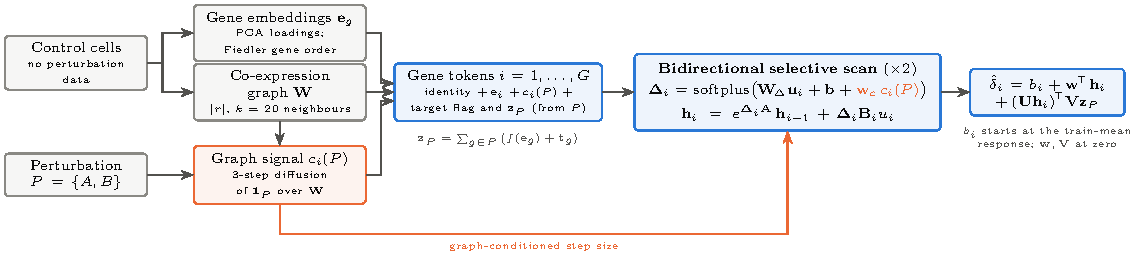
\includegraphics[width=\textwidth]{../manuscript/fig_arch.pdf}
\end{center}

\begin{enumerate}
\item \textbf{Inputs from control cells only} (no perturbation data leaks in): a co-expression graph,
a 64-number embedding of each gene, and a gene order along the graph (the Fiedler vector), so related genes
sit close in the sequence.
\item \textbf{Each of the 5,045 genes is a token.} A perturbation is added to the tokens in three ways:
a flag on the targeted genes; a summed embedding of the targets (so a gene never seen in training can still be
represented through its control-cell embedding); and the \emph{graph signal}, a 3-step diffusion of the
perturbation over the co-expression graph.
\item \textbf{Two layers of bidirectional selective scan.} The step size for every gene is
$\Delta_i=\mathrm{softplus}(\ldots+\mathbf{w}_c\,c_i(P))$, where $c_i(P)$ is large for genes near the
perturbed gene. \emph{This is the core idea.}
\item \textbf{Readout} starts exactly at the ``average response'' prediction and learns deviations. Without
this the model was no better than the mean in pilot runs.
\end{enumerate}
\textbf{Size and cost:} tiny --- width 32, state size 4, two layers; trains in about 7 minutes (median) to 17
minutes on a 4-core CPU. The scan is implemented in PyTorch as an exact chunked parallel scan and unit-tested
against a naive step-by-step version to $10^{-5}$.

\begin{callout}[title={\textbf{Say this if asked ``what is new?''}}]
The \emph{idea} (graph proximity modulating the SSM step size) is new to us as far as we know, but it turned
out not to help, so we do not claim it as a contribution that works. We claim: (i) a carefully controlled
negative result, (ii) the three pitfalls, and (iii) open code. Hedge on novelty --- ``as far as we know'' ---
and ask him whether the $R^2_{\mathrm{GI}}$ idea already exists elsewhere.
\end{callout}

% ============================================================
\section{How we tested it}

\subsection*{Data and splits}
\begin{itemize}
\item \textbf{Norman et al.\ 2019} (K562, CRISPRa): 91,205 cells, 5,045 genes, 7,353 control cells,
105 targeted genes, 131 doubles (GEO GSE133344).
\item \textbf{Adamson et al.\ 2016} (K562, CRISPRi): singles only, 86 perturbations, 5,060 genes
(GEO GSE90546; accession checked). 21 test perturbations per split.
\item \textbf{Splits:} the official GEARS ``simulation'' splits, seeds 1--5; each holds out about a quarter of
the targets. Across the five splits the Norman test sets have 185 unseen singles, 32 doubles with 0 seen,
254 with 1 seen, 90 with 2 seen (561 in all).
\end{itemize}

\subsection*{Baselines}
\begin{tabular}{@{}p{3.6cm}p{11.9cm}@{}}
\toprule
No change & Predict $\delta=0$.\\
Train mean & Predict the average response over training perturbations.\\
Additive & Sum of the targets' observed single responses (mean single response for an unseen target).\\
Linear (PCA) & Low-rank linear model of Ahlmann-Eltze et al.\ 2025; ridge penalty picked on validation data.\\
Linear (ctrl emb.) & Same, but using the control-cell gene embeddings our model gets.\\
GEARS & Official implementation, default settings; \textbf{split 1 only, 3 epochs} (about 40 min per epoch on CPU).\\
\bottomrule
\end{tabular}

\subsection*{Ablations (each removes or changes one thing)}
\begin{tabular}{@{}p{4.4cm}p{11.1cm}@{}}
\toprule
Variant & What it tests\\
\midrule
Mamba (no graph) & Is the graph needed at all?\\
Permuted graph & Does the \emph{content} of the graph matter, or only having some signal?\\
$\Delta$ only & Graph used only in the step size (the core idea), not also added to the tokens.\\
$\Delta$ only, random $\mathbf{w}_c$ & Same, but the conditioning weights start large, in case zero-initialisation hid an effect.\\
Random gene order & Does the graph-based gene ordering matter?\\
Graph-MLP (no scan) & Is the recurrence itself doing anything?\\
Additive prior (with/without graph) & Predict only the deviation from the additive sum: can a network add real
interaction information on top of additive?\\
\bottomrule
\end{tabular}

\subsection*{Metrics and statistics}
MSE and Pearson $r$ on each perturbation's top-20 DE genes; direction-of-change accuracy; $R^2_{\mathrm{GI}}$
for interactions on ``2/2 seen'' doubles. Five splits, mean $\pm$ s.d.; five variants trained from
\textbf{three random initialisations per split} (the other variants once); per-perturbation two-sided Wilcoxon
signed-rank tests pooled over splits with Holm correction within each metric and test group.

\subsection*{Model development}
All design decisions (readout, initialisation, learning rate) were made on the \emph{validation} perturbations
of split 1 only (Supplement Table S2); test perturbations were not used for that.

% ============================================================
\section{Results, with what to say about each}

\subsection*{7.1 Main table (Norman; MSE on top-20 DE genes; mean over five splits)}
\begin{center}\small
\begin{tabular}{@{}lccccc@{}}
\toprule
Model & Unseen single & 0/2 seen & 1/2 seen & 2/2 seen & All test\\
\midrule
No change & 0.346 & 0.752 & 0.669 & 0.647 & 0.561\\
Train mean & 0.270 & 0.576 & 0.511 & 0.485 & 0.428\\
Additive & 0.279 & 0.503 & 0.219 & \textbf{0.048} & \textbf{0.224}\\
Linear (PCA) & 0.269 & 0.616 & 0.400 & 0.296 & 0.349\\
\midrule
GCP-Mamba & \textbf{0.261} & 0.512 & 0.321 & 0.196 & 0.290\\
\ \ no graph & 0.265 & 0.513 & 0.301 & 0.169 & 0.278\\
\ \ permuted graph & 0.265 & 0.514 & 0.312 & 0.184 & 0.285\\
\ \ Graph-MLP (no scan) & 0.265 & 0.515 & 0.313 & 0.196 & 0.288\\
\ \ additive prior & 0.281 & 0.504 & 0.218 & \textbf{0.048} & 0.225\\
\bottomrule
\end{tabular}
\end{center}
Spread between splits is large (all-test s.d. 0.06--0.10), so differences of a few thousandths between
models are small next to it; the paired tests account for this.

\subsection*{7.2 Finding by finding}
\begin{enumerate}[label=\textbf{F\arabic*.},leftmargin=2em]
\item \textbf{Additive wins on doubles.} 0.224 overall; 0.048 for doubles with both singles seen versus 0.196
for our model ($P_{\mathrm{Holm}}<10^{-13}$).
\emph{Say:} ``This matches Ahlmann-Eltze et al.; for doubles whose singles you know, the sum is very hard to beat.''
\item \textbf{The graph does not help; it is slightly worse.} With vs without graph overall: 0.290 vs 0.278.
The graph-free model is slightly \emph{better}, statistically detectable
($P_{\mathrm{Holm}}=2\times10^{-5}$) but small (about 4\%). On unseen singles the two are equal (0.261 vs
0.265; not significant).
\emph{Say:} ``We can rule out a large benefit; we found none, and if anything a small cost on doubles.''
\item \textbf{The core mechanism (graph-conditioned step size) has no measurable effect.} $\Delta$-only equals
no-graph (0.279 vs 0.278); starting $\mathbf{w}_c$ large (norm $\approx5.8$) does not change that (0.276).
\item \textbf{Unseen singles: everything is within about 4\% of the mean.} 0.261--0.281 for all
methods except no-change (0.346) and the control-embedding linear model (0.322); GCP-Mamba is not significantly better than the train mean ($P_{\mathrm{Holm}}=0.42$),
the linear model ($P=1$), or the no-graph model ($P=1$).
\item \textbf{The recurrence adds nothing measurable} (Graph-MLP 0.288 vs 0.290; $P=0.83$); the Fiedler gene
order is no better than random order.
\item \textbf{No model captures interactions beyond additive.} $R^2_{\mathrm{GI}}$: additive-prior variants
$+0.01\pm0.02$ and $-0.01\pm0.06$ (i.e.\ zero); GCP-Mamba $-3.04$; no-graph $-2.51$; train mean $-9.10$;
no change $-12.54$; GEARS $-3.5$ on split 1 (19 doubles).
\item \textbf{GEARS is best on unseen genes (split 1 only, 3 epochs).} Unseen singles 0.214 vs 0.262 for
GCP-Mamba and 0.247 for the train mean; overall 0.230 vs 0.269 for GCP-Mamba ($P_{\mathrm{Holm}}=0.003$,
$n=107$); additive still best overall on that split (0.213).
\emph{Say:} ``This supports our explanation that the co-expression graph is the weak part, but it is one split
and shortened training, so we call it indicative.''
\item \textbf{Adamson: nothing beats the mean.} All methods except no-change: 0.161--0.171 (mean baseline
0.171; s.d.\ across splits 0.05--0.07). Consistent with Csendes et al.\ (2025), who found perturbation-specific
variance is low in these benchmark datasets.
\item \textbf{Cost.} The scan grows about linearly: 0.15\,s/0.23\,GB at 500 genes, 3.1\,s/1.6\,GB at 5,000,
16.8\,s/6.0\,GB at 20,000. Dense attention needed 3.5\,GB at 2,000 genes and ran out of 15\,GB at 5,000. But a
sparse graph network (GEARS-like) was 6--25$\times$ faster and used 25--50$\times$ less memory than the scan.
\emph{Say this yourselves:} SSMs make transcriptome-wide tokens feasible where attention isn't, but they are not
more efficient than sparse GNNs.
\end{enumerate}

\begin{callout}[title={\textbf{How to phrase ``no effect''}}]
``Not significant'' is not ``proven zero.'' The honest phrasing is: \emph{we found no measurable effect, and the
differences we can see are within about 2--4\% of the error, smaller than the between-split spread and than
random-initialisation noise.} That claim is defensible; ``the graph is useless'' is not.
\end{callout}

% ============================================================
\section{The three pitfalls (the paper's main contribution)}

\subsection*{Pitfall 1: an input encoding tied to the output genes silently discarded most perturbations}
\begin{itemize}
\item First version: a perturbation was a 0/1 vector over the 500 most variable genes (the same genes being
predicted); single perturbations written \texttt{ctrl+GENE} were read as ``control.''
\item Only \textbf{12--17 of the 105} targeted genes were among those 500 (mean 14 over ten splits). So
\textbf{77--84\% (mean 80\%) of training} and 70--94\% of test perturbations became all-zero inputs; the
161--183 training perturbations of a split shared only 14--19 distinct inputs.
\item Consequence: the model could at best learn the average response; the old ``the graph doesn't help''
conclusion said nothing about the architecture. Training looked normal (loss decreased), which is why it was
easy to miss.
\item Evidence: Supplement Table S1, script \texttt{gcpm/audit\_hvg\_encoding.py}, legacy code in \texttt{legacy/}.
\item \textbf{Takeaway:} report how many perturbation targets actually reach the model input.
\end{itemize}

\subsection*{Pitfall 2: a single-seed comparison suggested a graph effect that was not there}
\begin{itemize}
\item In an earlier run with one initialisation per split, GCP-Mamba looked significantly better than both
graph controls on unseen singles.
\item Re-initialising GCP-Mamba alone changed its unseen-single error from 0.255 to 0.261 --- the same size as the
supposed effect. With three initialisations averaged, the difference vanished.
\item Within a split, the same model's error varies by about 0.024 (s.d.) and 0.046 (range) between
initialisations (Supplement Table S4).
\item \textbf{Takeaway:} use several initialisations before claiming a small effect.
\end{itemize}

\subsection*{Pitfall 3: the genetic-interaction Pearson correlation ranks models in reverse}
\begin{itemize}
\item Earlier work scores GI prediction by the correlation between predicted and true \emph{residuals}
($\delta_{AB}-\delta_A-\delta_B$).
\item On ``2/2 seen'' doubles this gives our additive-prior models (which are essentially exact) \textbf{0.14
and 0.20}, but gives the models that explain \emph{least} interaction the highest scores: GCP-Mamba 0.36,
no-graph 0.37, GEARS 0.38 (split 1 only) --- and even ``no change'' 0.25 and ``train mean'' 0.28.
\item \emph{Why:} predicting no change gives a predicted residual of $-(\delta_A+\delta_B)$, which is correlated
with the true residual whenever the interaction is buffering (sub-additive). Any prediction shrunk towards zero
inherits that correlation.
\item Our fix: $R^2_{\mathrm{GI}}=1-\sum \mathrm{MSE}/\sum \overline{\epsilon^2}$, the fraction of interaction
variance explained; additive $=0$ by construction.
\item \textbf{Takeaway:} don't use a correlation of residuals alone. \emph{Note for honesty:} the ``why'' is an
argument plus the empirical pattern; we did not write a formal proof or a simulation (a good follow-up).
\end{itemize}

\begin{center}
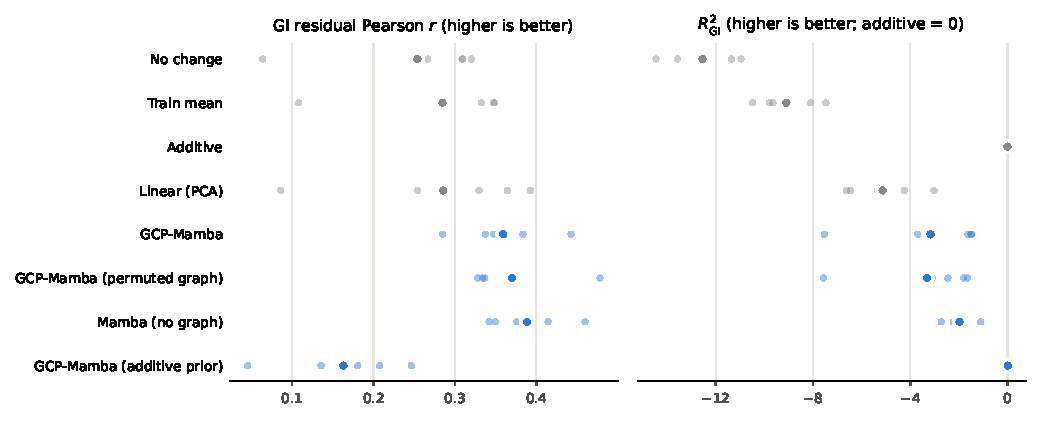
\includegraphics[width=0.92\textwidth]{../manuscript/fig_gi.pdf}
\end{center}
\textit{How to read the figure:} left, the correlation (higher looks better) rates trained models above the
additive-prior models; right, variance explained (0 = additive) shows the opposite. Grey = baselines, blue =
our model and variants; big dot = mean over splits, small dots = individual splits.

% ============================================================
\section{How the project got here (so you can tell it straight)}
\begin{enumerate}
\item \textbf{Original draft:} reported that graph conditioning did not help,
with a GEARS row that was not a rerun (it was labelled as cited from the GEARS paper, and its values coincided with our own
deep models' values) and several numbers that disagreed between abstract, text and tables. It also contained a placeholder
``received/accepted'' history line; \textbf{the paper has not been submitted or accepted anywhere}, and that
line has been removed. If Anthony has seen an older copy, that is why it differs.
\item \textbf{Audit:} on the authors' own data file (checksum matched) we found the input-encoding problem
(Pitfall 1).
\item \textbf{Rebuild:} new model and pipeline (every target represented, gene- and perturbation-specific graph
signal, bidirectional scan over all genes, train-mean initialisation), standard GEARS splits, proper baselines,
ablations, seeds, tests, a second dataset.
\item \textbf{Two rounds of self-correction:} an early-stopping rule that had cut some runs off unfairly
(now a 40-epoch minimum, affected runs rerun), and the seed effect (Pitfall 2), which is why the final
model variants use three initialisations.
\item \textbf{Result:} the original ``it doesn't help'' conclusion survived, but now it is supported.
\end{enumerate}

\begin{callout}[title={\textbf{If he asks ``so was your first paper wrong?''}}]
``Its conclusion turned out to be right for a wrong reason. The model was being fed all-zero inputs for most
perturbations, so its result said nothing about the architecture. We found the bug, rebuilt everything, and
re-tested; the conclusion held, and now we have controls that support it. We wrote the bug up because we think
other people could make the same mistake.''
\end{callout}

% ============================================================
\section{Weak points a careful reader will find --- and honest answers}

\begin{tabular}{@{}p{4.1cm}p{11.4cm}@{}}
\toprule
Weak point & What to say\\
\midrule
GEARS: 1 split, 3 of 20 epochs & Compute-limited (CPU only; 40 min/epoch). Its built-in logging evaluations
were skipped to fit in 15\,GB RAM; predictions are scored exactly like all other models. Called ``indicative''
in the paper. A GPU rerun on all five splits is the top improvement.\\
Only K562, two screens & True. The doubles claim rests on one dataset (Norman). Replogle screens were excluded
because most of their targets are not measured genes in the GEARS release, which our per-gene-token encoding
needs. Ask for a better dataset.\\
No noise ceiling & We did not estimate how well any model could do (e.g.\ split-half reproducibility). That is
a gap; a reviewer may ask. Adding it is feasible with the current data.\\
Tuning fairness & GCP-Mamba's design was tuned on split-1 validation only; ablations were not tuned
separately; linear baselines' ridge penalty was tuned on validation; GEARS used defaults. None of the variants
came near the additive baseline, so tuning is unlikely to reverse the conclusion --- but it is a fair
question.\\
Statistics & Pooled Wilcoxon tests treat perturbations as independent although the same perturbation can occur
in several overlapping splits; we say the tests are approximate and stress effect sizes. A mixed-effects
model or per-split tests would be cleaner --- ask him.\\
Low power on interactions & Only 19--90 test doubles in the ``2/2 seen'' group; $R^2_{\mathrm{GI}}\approx0$ means
``no evidence of beating additive,'' not ``interactions are unpredictable.''\\
Additive-prior variants & They match additive \emph{by construction} at the start; the informative result is that
training never moved them meaningfully away from it (they learned a negligible correction).\\
Graph choices untuned & $k=20$, three diffusion steps, decay 0.5 were fixed a priori. A better or different graph
(Gene Ontology, protein interactions) is the obvious next experiment.\\
Reproducibility & Code and per-perturbation results are public; predictions are saved locally but the planned
Zenodo deposit has \textbf{not} been made yet.\\
Same authors wrote the bug & Say so openly; that is the point of Pitfall 1.\\
\bottomrule
\end{tabular}

\begin{warning}[title={\textbf{Be ready for: ``who wrote the code / the paper?''}}]
This revision (audit, rebuilt model, experiments, tables, figures, manuscript text) was produced with
substantial help from Claude, an AI coding assistant, working from your instructions. Whatever the exact
division of work, \textbf{you must be able to explain and defend every part}: read the model file
(\texttt{gcpm/model.py}), the benchmark (\texttt{gcpm/benchmark.py}) and Section~2 of the paper until you can
walk through them. Also: the earlier draft had an ``AI use disclosure''; the current draft does not, and the
author-contributions statement was written without knowing exactly who did what. Check the journal's policy
on disclosing AI assistance, then add an accurate disclosure and contribution statement before submitting. Be
straightforward if Anthony asks.
\end{warning}

% ============================================================
\section{Likely questions, with answers}

\subsection*{The science and biology}
\qa{Why is additive so hard to beat?}{For a double whose two singles you have measured, most of the response
is literally the sum. Interactions are a small correction on top, so a model has to predict a small,
noisy difference. Ahlmann-Eltze et al.\ report the same for other deep models.}
\qa{Do you see real genetic interactions in these data?}{Yes --- Norman et al.\ characterised strong ones. Our
statement is only that none of \emph{our models} (or GEARS on split 1) predict the interaction part better
than assuming additivity.}
\qa{Why the top-20 DE genes?}{It is the GEARS/standard convention: most of the 5,045 genes barely change, so
all-gene error is dominated by noise. We also computed Pearson correlation on the same genes (Supplement Table S5) and
direction-of-change accuracy (\texttt{results/summary\_direction\_de20.csv}); the ranking of methods is similar.}
\qa{CRISPRa vs CRISPRi --- does it matter?}{Norman uses activation, Adamson interference. We use both to
check the conclusions are not specific to one; Adamson has only singles, so it cannot test interactions.}

\subsection*{The model}
\qa{Why a state-space model for genes?}{Linear time and memory in the number of genes, so all 5,045 (and in
principle 20,000) genes can be tokens. Attention ran out of memory at 5,000 on our machine.}
\qa{Genes have no order --- isn't a sequence model wrong?}{That was one of our worries. We order genes along
the graph so related genes are neighbours and use a bidirectional scan; a random order performed the same, and
a no-recurrence MLP performed the same, so the sequence machinery does not appear to matter here.}
\qa{How exactly does the graph enter?}{We diffuse the perturbation over the co-expression graph for three steps
to get a per-gene signal $c_i(P)$ and add $\mathbf{w}_c c_i(P)$ inside the softplus that sets each gene's step
size (and also add the signal to the token features in the full model).}
\qa{Could the model just be under-trained or badly tuned?}{We watched for that: validation curves, minimum
40 epochs, and a variant starting the graph weights large. All variants converge to similar error, and the
additive-prior variants recover the additive baseline, which shows the pipeline can reach a good solution.}
\qa{How do you know the scan is correct?}{A unit test compares it to a naive step-by-step implementation to
$10^{-5}$ (\texttt{tests/test\_scan.py}).}

\subsection*{Statistics and evaluation}
\qa{Are your tests valid?}{They are approximate: we pool perturbations across splits and use paired Wilcoxon
tests with Holm correction; the same perturbation can appear in several splits. We emphasise effect sizes and
consistency across splits. We would welcome advice on a mixed-effects alternative.}
\qa{Why three seeds and only for some variants?}{Compute. The five variants that matter for the main claims
(full model, permuted graph, no graph, no recurrence, additive prior) have three; others one. The seed
variation is reported in Supplement Table S4.}
\qa{Is $R^2_{\mathrm{GI}}$ new?}{Not that we know of in this literature, but we would not claim novelty
without checking --- is it standard in another field?}
\qa{What about a noise ceiling?}{Not done; it is on the to-do list (e.g.\ split-half reproducibility of the
measured responses).}

\subsection*{Framing, venue and practicalities}
\qa{Is a negative result publishable?}{As a careful evaluation with reusable pitfalls, it can be; we are not
assuming acceptance. That is exactly what we want advice on.}
\qa{Would you resubmit with a positive result if you tried a different graph?}{Possibly as a follow-up; the
current paper stands on its own as an evaluation. We would not tune until the model wins.}
\qa{Why only two authors, both students?}{Riley led biology and writing; Aryan led the modelling and
experiments. We are seeking mentorship and feedback, not a co-author to add credibility.}
\qa{Where is the code?}{\url{https://github.com/The-MathKing/gcpmamba} (MIT license) --- but see the warning on
page~1 about which branch to point to. \texttt{README.md} explains how to reproduce everything;
\texttt{python -m gcpm.report} regenerates every table and figure.}

% ============================================================
\section{Questions to ask him}

\begin{tabular}{@{}p{0.6cm}p{8.4cm}p{6.5cm}@{}}
\toprule
\# & Question & What to listen for\\
\midrule
1 & Is a careful negative result plus evaluation pitfalls a good fit for \emph{Bioinformatics}? Would
\emph{Bioinformatics Advances}, \emph{PLOS Comp.\ Biol.} or an ML-for-biology workshop suit it better? Should we
post a bioRxiv preprint first? & Specific venues, and what makes editors take a negative-result paper.\\
2 & Should we lead with the model or with the pitfalls (especially the metric reversal)? & Whether he finds the
pitfalls or the model more interesting.\\
3 & How much does the reduced GEARS run (1 split, 3 epochs) weaken the paper? Where could high-school students
get GPU time? & Concrete compute options; whether a citation would suffice.\\
4 & GEARS's Gene Ontology graph helped on unseen genes. Should we swap in GO or STRING and rerun, or is that a
different paper? & Whether he sees a natural sequel.\\
5 & Is our statistical approach acceptable, or should we use per-split tests or a mixed model? & A named method or
reference.\\
6 & Is $R^2_{\mathrm{GI}}$ sound, or is there an established alternative? & Prior work we missed.\\
7 & Is there another combinatorial screen or a standard way to use the Replogle data? & Datasets, or advice on
scoping down.\\
8 & What is the single analysis a reviewer would insist on that we do not have? & His top priority --- write it down.\\
9 & Would you be willing to look at a revised draft in a few weeks? & A yes/no; be gracious about either.\\
\bottomrule
\end{tabular}

\subsection*{Etiquette}
\begin{itemize}
\item Ask for \textbf{feedback and pointers}, not authorship or submission help.
\item If he suggests something outside your reach (e.g.\ big compute), ask ``what is the smallest version of
that we could do?''
\item End by restating his 2--3 suggestions so he can correct you.
\end{itemize}

% ============================================================
\section{During and after the call}

\subsection*{Note-taking template}
\begin{tabular}{@{}p{4cm}p{11.5cm}@{}}
\toprule
Venue advice & \\[14pt]
Analyses he says are required & \\[14pt]
Compute / dataset leads & \\[14pt]
Papers or people to look up & \\[14pt]
His reaction to the framing & \\[14pt]
Follow-ups (who does what by when) & \\[14pt]
\bottomrule
\end{tabular}

\subsection*{Thank-you email (send within a day)}
\begin{quote}
Hi Anthony,\\
Thank you again for your time and for the thoughtful feedback. The points we took away were: [1], [2], [3].
We'll work on those and, if you're open to it, would love to send you a revised draft in [timeframe].
Thanks also to Kevin for the introduction.\\
Best,\\ Riley [and Aryan]
\end{quote}

% ============================================================
\section{Before you submit anywhere (open items)}
\begin{itemize}
\item \textbf{Merge or repoint the repository link} (page~1 warning). Decide on a tagged release.
\item \textbf{AI-assistance disclosure and author-contributions statement:} make both accurate; check the
journal's current policy (Section~9 box).
\item \textbf{Zenodo deposit} of predictions (the paper says it ``will be deposited''). Either do it or remove
the sentence.
\item Fill template placeholders: Associate Editor, dates, corresponding-author details; check affiliations.
\item Verify each reference and data accession against the source once more (checked: Adamson et al.\ 2016 and its
accession GSE90546, Ahlmann-Eltze et al.\ 2025, Csendes et al.\ 2025, the TxPert publication; \textbf{not yet
checked:} the Norman accession GSE133344 and the volume/page numbers of the remaining references).
\item Optional but valuable: GEARS on all 5 splits (GPU), noise ceiling, a small simulation of the Pearson
reversal, per-split or mixed-model statistics, a knowledge-graph variant.
\end{itemize}

% ============================================================
\appendix
\section{Key numbers on one page}

\begin{center}\small
\begin{tabular}{@{}p{7.2cm}p{8.3cm}@{}}
\toprule
\textbf{Fact} & \textbf{Value}\\
\midrule
Norman: cells / genes / controls / singles / doubles & 91,205 / 5,045 / 7,353 / 105 / 131 (of 5,460 pairs)\\
Test perturbations (5 splits) & 185 unseen singles, 32 (0/2), 254 (1/2), 90 (2/2) = 561\\
Adamson & 86 singles, 5,060 genes, 21 test perturbations per split\\
Models trained (Norman, deep) & up to 3 initialisations $\times$ 5 splits per main variant\\
Additive, all / 2-of-2 seen & 0.224 / 0.048\\
GCP-Mamba, all / 2-of-2 seen & 0.290 / 0.196\\
No-graph Mamba, all & 0.278 (vs GCP-Mamba: $P_{\mathrm{Holm}}=2\times10^{-5}$, graph-free better)\\
Train mean / linear / no change, all & 0.428 / 0.349 / 0.561\\
Unseen singles: GCP-Mamba / mean / additive / GEARS (split 1) & 0.261 / 0.270 / 0.279 / 0.214 (GCP-Mamba on split 1: 0.262)\\
$R^2_{\mathrm{GI}}$: additive-prior / GCP-Mamba / no graph / train mean / no change & $\approx0$ / $-3.04$ / $-2.51$ / $-9.10$ / $-12.54$\\
GI Pearson: additive-prior / GCP-Mamba / GEARS / no change & 0.14 / 0.36 / 0.38 / 0.25\\
Adamson, all except no change & MSE 0.161--0.171 (train mean 0.171)\\
Initialisation noise (GCP-Mamba, within split) & s.d.\ 0.024, range 0.046\\
Legacy encoding & 12--17 of 105 targets in the 500 genes; 77--84\% of training inputs all-zero (mean 80\%)\\
Scan cost: 500 / 5,000 / 20,000 genes & 0.15\,s, 0.23\,GB / 3.1\,s, 1.6\,GB / 16.8\,s, 6.0\,GB\\
Attention memory & 3.5\,GB at 2,000 genes; out of memory (15\,GB) at 5,000\\
Model size / training time & width 32, state 4, 2 layers; median 7 min, max 17 min per run (4-core CPU)\\
GEARS run & split 1, 3 of 20 epochs, about 40 min/epoch (test-set logging evaluation skipped for memory)\\
\bottomrule
\end{tabular}
\end{center}

\section{Reading list (skim in this order)}
\begin{enumerate}
\item Ahlmann-Eltze, Huber, Anders (2025), \emph{Deep-learning-based gene perturbation effect prediction does
not yet outperform simple linear baselines}, \emph{Nat.\ Methods} 22:1657--1661,
\url{https://doi.org/10.1038/s41592-025-02772-6}. \textbf{The paper ours builds on --- read the abstract and
figures.}
\item Roohani, Huang, Leskovec (2024), \emph{GEARS}, \emph{Nat.\ Biotechnol.} 42:927--935: the model we compare with
and the source of the splits.
\item Norman et al.\ (2019), \emph{Science} 365:786--793: the dataset and what genetic interactions look like.
\item Csendes et al.\ (2025), \emph{BMC Genomics} 26:393, \url{https://doi.org/10.1186/s12864-025-11600-2}: the mean
baseline beats foundation models; benchmark datasets have low perturbation-specific variance.
\item Gu \& Dao (2023), \emph{Mamba}, arXiv:2312.00752: only the introduction and the selective-scan idea.
\item Wenkel et al.\ (2026), \emph{TxPert}, \emph{Nat.\ Biotechnol.}: uses several knowledge graphs, relevant to the
``try a better graph'' next step.
\end{enumerate}

\section{Where things are (repository map)}
\begin{tabular}{@{}p{5.4cm}p{10.1cm}@{}}
\toprule
\texttt{manuscript/main.pdf} & the 7-page paper (Bioinformatics template); \texttt{supplementary.pdf} is 4 pages\\
\texttt{manuscript/BRIEFING.md} & shorter briefing\\
\texttt{meeting/} & one-page summary, reply-email draft, call prep, and this document\\
\texttt{gcpm/model.py} & the model and the parallel scan\\
\texttt{gcpm/benchmark.py} & baselines, variants, training, metrics\\
\texttt{gcpm/report.py} & regenerates all tables and figures\\
\texttt{results/} & per-perturbation metrics for every model and split\\
\texttt{legacy/} & the first version and its manuscript (kept for transparency)\\
\texttt{tests/test\_scan.py} & scan correctness test\\
\bottomrule
\end{tabular}

\end{document}
